\documentclass[spanish,letterpaper,oneside]{article}

% Datos del documento
\def\documenttitle {Distancia entre puntos del plano cartesiano}
\def\documentsubtitle {Temas selectos de matemáticas I}
\def\documentsubject {Actividad 10 · Resolución del modelo y reflexión pedagógica}
\def\documentauthor {Mtro. Martín Jonathan de la Cruz Muñoz}
\def\coursename {Temas selectos de matemáticas I}
\def\coursecode {PFM02}

% Identidad institucional
\def\universityname {Instituto de Investigación, Innovación y Estudios de Posgrado para la Educación del Estado de Nuevo León}
\def\universityfaculty {Maestría en Aprendizaje y Enseñanza de las Matemáticas}
\def\universitydepartment {Temas selectos de matemáticas I}
\def\universitydepartmentimage {img/iiiepe/marca-iiiepe.png}
\def\universitydepartmentimagecfg {height=1.75cm}
\def\universitylocation {Monterrey, Nuevo León}
\def\studentfullname {Mtro. Martín Jonathan de la Cruz Muñoz}
\def\studentid {00874}
\def\studentemail {martin.delacruz@campus.iiiepe.edu.mx}
\def\programperiod {1er tetramestre, marzo--julio de 2026}
\def\programmodality {Modalidad presencial}
\def\programshort {MAEM}

\def\authortable {
  \begin{tabular}{ll}
    \textbf{Alumno:} & \studentfullname \\
    Matrícula: & \studentid \\
    Correo institucional: & \studentemail \\
    Unidad: & \coursename \\
    Programa: & \programshort \\
    Periodo: & \programperiod \\
    & \\
    \multicolumn{2}{l}{Fecha de realización: 13 de octubre de 2026} \\
    \multicolumn{2}{l}{\universitylocation}
  \end{tabular}
}

\input{template}

\usepackage{helvet}
\renewcommand{\familydefault}{\sfdefault}
\usepackage{array}
\usepackage{longtable}
\usepackage{pdflscape}
\usepackage{tikz}
\usepackage[most]{tcolorbox}
\usetikzlibrary{arrows.meta,positioning,calc,fit,backgrounds}

\definecolor{iiiepeNavy}{HTML}{163B5C}
\definecolor{iiiepeBlue}{HTML}{1F6F9F}
\definecolor{iiiepeAqua}{HTML}{20B7A8}
\definecolor{iiiepeOrange}{HTML}{F28C28}
\definecolor{iiiepePaper}{HTML}{F6F8F7}
\definecolor{iiiepeInk}{HTML}{1E2A32}
\def\portraittitlecolor {iiiepeNavy}
\setcitestyle{authoryear,open={(},close={)}}

\newcommand{\insertcoverwatermark}{%
  \AddToShipoutPictureBG*{%
    \begin{tikzpicture}[remember picture,overlay]
      \node[opacity=.09,inner sep=0pt] at (current page.center)
      {\includegraphics[width=.58\paperwidth]{img/iiiepe/logo-puntos.png}};
    \end{tikzpicture}%
  }%
}

\newtcolorbox{reportelecturabox}[1][]{%
  enhanced,breakable,
  colback=iiiepePaper,colframe=iiiepeNavy,
  boxrule=1pt,leftrule=4pt,arc=2pt,
  left=8pt,right=8pt,top=6pt,bottom=6pt,
  before skip=6pt,after skip=10pt,
  fonttitle=\bfseries\color{white},coltitle=white,
  colbacktitle=iiiepeNavy,
  attach boxed title to top left={xshift=8pt,yshift=-2pt},
  boxed title style={colback=iiiepeNavy,colframe=iiiepeNavy,arc=1pt},
  title={Reporte de lectura},#1}

\newtcolorbox{fichalecturabox}[1][]{%
  enhanced,breakable,
  colback=iiiepeAqua!7,colframe=iiiepeAqua!70!iiiepeNavy,
  boxrule=.6pt,arc=1pt,
  left=7pt,right=7pt,top=4pt,bottom=4pt,
  fontupper=\small,before upper={\setstretch{1.0}},
  fonttitle=\bfseries\color{iiiepeNavy},coltitle=iiiepeNavy,
  colbacktitle=iiiepeAqua!7,
  title={Ficha de la lectura},#1}



\usepackage{tabularx,colortbl,pgfplots,enumitem,needspace}\pgfplotsset{compat=1.18}\definecolor{iiiepePale}{HTML}{EEF5F8}
\setlength{\parskip}{5pt}\setlength{\parindent}{0pt}
\begin{document}\insertcoverwatermark\templatePortrait\templatePagecfg\templateFinalcfg\fancyfoot{}\fancyfoot[L]{\scriptsize IIIEPE · MAEM}\fancyfoot[C]{\scriptsize\thepage}\fancyfoot[R]{\scriptsize Actividad 10}\setstretch{1.3}\raggedbottom
\section{Distancia como longitud de un segmento}
La distancia entre dos puntos del plano se obtiene construyendo un triángulo rectángulo con las diferencias de coordenadas como catetos. No se suman directamente las coordenadas: se calcula la longitud del segmento que une los puntos.
\[
d(A,B)=\sqrt{(x_B-x_A)^2+(y_B-y_A)^2}.
\]
La distancia siempre es no negativa y tiene la misma unidad que las coordenadas. La fórmula requiere ejes perpendiculares y la misma escala física en ambos.
\section{Registro y resolución}
La ficha solicita registrar tres lanzamientos reales desde una catapulta ubicada en $(0,0)$. El ejemplo oficial $(120,50)$ permite comprobar $d=\sqrt{120^2+50^2}=130$ cm. Las filas siguientes son \textbf{datos simulados para desarrollar el método}; no se confunden con los lanzamientos reales, disponibles como referencia cualitativa.


{\small\setstretch{1.1}\renewcommand{\arraystretch}{1.25}
\begin{longtable}{|>{\raggedright\arraybackslash}p{\dimexpr0.3\linewidth-2\tabcolsep-2\arrayrulewidth\relax}|>{\raggedright\arraybackslash}p{\dimexpr0.35\linewidth-2\tabcolsep-2\arrayrulewidth\relax}|>{\raggedright\arraybackslash}p{\dimexpr0.35\linewidth-2\tabcolsep-2\arrayrulewidth\relax}|}\hline
\rowcolor{iiiepePale} \textbf{Punto} & \textbf{Coordenadas (cm)} & \textbf{Distancia al origen} \\\hline
\endfirsthead
\hline
\rowcolor{iiiepePale} \textbf{Punto} & \textbf{Coordenadas (cm)} & \textbf{Distancia al origen} \\\hline
\endhead
A & $(120,50)$ & $130$ cm \\\hline
B & $(80,20)$ & $\sqrt{6800}=20\sqrt{17}\approx82.46$ cm \\\hline
C & $(100,-30)$ & $\sqrt{10900}=10\sqrt{109}\approx104.40$ cm \\\hline
\end{longtable}}


La distancia entre A y B es $\sqrt{(80-120)^2+(20-50)^2}=\sqrt{1600+900}=50$ cm. Entre A y C, $\sqrt{(-20)^2+(-80)^2}=20\sqrt{17}\approx82.46$ cm. Entre B y C, $\sqrt{20^2+(-50)^2}=10\sqrt{29}\approx53.85$ cm.
\begin{center}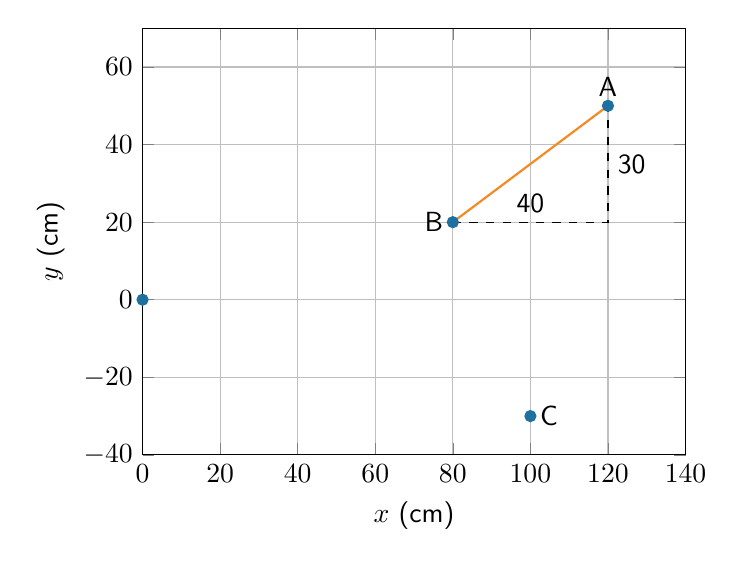
\begin{tikzpicture}\begin{axis}[width=11cm,height=7cm,axis equal image,xmin=0,xmax=140,ymin=-40,ymax=70,xlabel={$x$ (cm)},ylabel={$y$ (cm)},grid=major]
\addplot[only marks,mark=*,iiiepeBlue] coordinates {(0,0)(120,50)(80,20)(100,-30)};
\addplot[thick,iiiepeOrange] coordinates {(80,20)(120,50)};\addplot[dashed] coordinates {(80,20)(120,20)(120,50)};
\node[above] at (axis cs:120,50){A};\node[left] at (axis cs:80,20){B};\node[right] at (axis cs:100,-30){C};\node[above] at (axis cs:100,20){40};\node[right] at (axis cs:120,35){30};
\end{axis}\end{tikzpicture}\end{center}
\section{Deducir la fórmula y comprobar el resultado}
Entre $A=(120,50)$ y $B=(80,20)$, el cambio horizontal tiene magnitud $|120-80|=40$ cm y el vertical $|50-20|=30$ cm. Los ejes perpendiculares permiten aplicar Pitágoras: $d^2=40^2+30^2=2500$, por lo que $d=50$ cm. Sumar 40 y 30 da la longitud de una ruta por los ejes, 70 cm; no la del segmento directo.
La fórmula conserva simetría: intercambiar A y B cambia los signos de las diferencias, pero sus cuadrados permanecen iguales. También produce distancia cero si los dos puntos coinciden. Estas comprobaciones son más informativas que memorizar la expresión sin interpretar sus componentes.


\subsection{Referencia cualitativa a los lanzamientos}
Se dispone de mediciones de los lanzamientos. Su lectura cualitativa se centra en la definición del origen, el sentido de los ejes, la coherencia entre coordenadas y posición y la comparación entre distancia calculada y medida directa. La referencia a estas pruebas permite vincular la fórmula con el proceso de medir, sin atribuir una concordancia numérica que no se transcribe aquí. Los puntos del ejemplo siguen siendo un recurso de demostración matemática.

\section{Secuencia de aplicación y evaluación}
Deducir y aplicar la distancia cartesiana. La duración propuesta es de 90 minutos, ajustable al diagnóstico y a los recursos. Esta planeación sigue la progresión de los recursos institucionales (IIIEPE, 2026); los tiempos y apoyos son decisiones de codiseño, no datos de una aplicación ya realizada.

{\small\setstretch{1.1}\renewcommand{\arraystretch}{1.25}
\begin{longtable}{|>{\raggedright\arraybackslash}p{\dimexpr0.23\linewidth-2\tabcolsep-2\arrayrulewidth\relax}|>{\raggedright\arraybackslash}p{\dimexpr0.49\linewidth-2\tabcolsep-2\arrayrulewidth\relax}|>{\raggedright\arraybackslash}p{\dimexpr0.28\linewidth-2\tabcolsep-2\arrayrulewidth\relax}|}\hline
\rowcolor{iiiepePale} \textbf{Fase y tiempo} & \textbf{Actividad y mediación} & \textbf{Evidencia} \\\hline
\endfirsthead
\hline
\rowcolor{iiiepePale} \textbf{Fase y tiempo} & \textbf{Actividad y mediación} & \textbf{Evidencia} \\\hline
\endhead
1. Reto y saberes (10 min) & Comparar una ruta por los ejes con el segmento directo. & Predicción individual y pregunta. \\\hline
2. Plan de indagación (15 min) & Fijar origen, escala y registro antes de los lanzamientos. & Plan explicado y criterios. \\\hline
3. Construcción y análisis (30 min) & Medir tres impactos y construir triángulos entre puntos. & Registro o procedimiento trazable. \\\hline
4. Comunicación y aplicación (20 min) & Aplicar Pitágoras y contrastar una distancia con medición directa. & Argumento con comprobación. \\\hline
5. Metacognición (15 min) & Explicar diferencias de registro y transferir a una placa de taller. & Versión revisada y justificación. \\\hline
\end{longtable}}
\subsection{Criterios observables y retroalimentación}

{\small\setstretch{1.1}\renewcommand{\arraystretch}{1.25}
\begin{longtable}{|>{\raggedright\arraybackslash}p{\dimexpr0.22\linewidth-2\tabcolsep-2\arrayrulewidth\relax}|>{\raggedright\arraybackslash}p{\dimexpr0.4\linewidth-2\tabcolsep-2\arrayrulewidth\relax}|>{\raggedright\arraybackslash}p{\dimexpr0.38\linewidth-2\tabcolsep-2\arrayrulewidth\relax}|}\hline
\rowcolor{iiiepePale} \textbf{Criterio} & \textbf{Evidencia de logro} & \textbf{Acción si necesita apoyo} \\\hline
\endfirsthead
\hline
\rowcolor{iiiepePale} \textbf{Criterio} & \textbf{Evidencia de logro} & \textbf{Acción si necesita apoyo} \\\hline
\endhead
Registro y referencia & Explica registro y referencia con un caso de la actividad. & Pedir una representación concreta y contrastar dos casos. \\\hline
Ubicación cartesiana & Conserva ubicación cartesiana en el desarrollo y justifica sus pasos. & Modelar un paso, retirar gradualmente la ayuda y solicitar otro caso. \\\hline
Pitágoras & Utiliza pitágoras para contrastar una respuesta o representación. & Comparar la evidencia inicial y la corregida con una pregunta específica. \\\hline
Interpretación del error & Relaciona interpretación del error con la conclusión y un límite del problema. & Solicitar una comprobación independiente y un caso de transferencia. \\\hline
\end{longtable}}
El instrumento es una propuesta docente. Cada criterio se registra como logrado con autonomía, logrado con apoyo o aún no demostrado; no se asigna una calificación observada sin aplicar la actividad. En la coevaluación, un compañero verifica un criterio y formula una pregunta; en la autoevaluación, el estudiante explica una corrección; el docente contrasta ambas evidencias y decide el siguiente apoyo.\subsection{Participación y apoyos}
La inclusión se concreta en alternativas de representación y de acceso; el pensamiento crítico, en justificar y contrastar. Los roles de cálculo, registro y explicación se rotan para que todos produzcan una evidencia individual. Quien necesita apoyo dispone de un ejemplo parcial y preguntas graduadas; quien ya domina el procedimiento analiza un contraejemplo o cambia una condición. Estas acciones deben observarse durante la aplicación para valorar su funcionamiento.

\section{Reflexión pedagógica}
Si el tiempo no alcanza, dejaría para casa la representación gráfica y la explicación de una distancia, después de verificar en clase que se comprenden los ejes y las unidades. La revisión pediría resolver un caso nuevo y justificar el triángulo utilizado; recibir un archivo no basta para comprobar comprensión. Ofrecería una alternativa en papel para quienes no tengan acceso digital.
Como aplicación alternativa, usaría la separación entre dos puntos de fijación en una placa de taller. También puede marcarse un plano con cinta en el piso y pedir una ruta directa y una ruta por los ejes. La segunda mide $|\Delta x|+|\Delta y|$, que generalmente excede la distancia euclidiana; comparar ambas ayuda a comprender el teorema de Pitágoras.
Rediseñaría la catapulta para usar proyectiles blandos, delimitar el área y asignar tareas accesibles de medición, registro y comprobación. Si repitiera el diseño, fijaría el origen, acordaría el sentido positivo de cada eje y registraría incertidumbre antes de calcular. Son mejoras propuestas; no se declara una ejecución física previa.
\section{Evaluación formativa e interpretación de evidencia}
Quedan resueltos los cálculos y la representación del ejemplo. Las mediciones existentes son la referencia de la parte experimental; en este reporte se presenta su lectura cualitativa. La validación numérica de tres pares de coordenadas requiere consultar el registro original. La lista de cotejo revisaría identificación de ejes, registro, ubicación de puntos, formación del triángulo, uso de la fórmula y explicación; la autoevaluación se completa con la evidencia real.

\needspace{5\baselineskip}\section*{Referencias}
{\setstretch{1.15}\setlength{\parskip}{6pt}
\par\hangindent=1.27cm\hangafter=1  Academia Estatal de Matemáticas. (2023). \textit{Practicando saberes en Matemáticas: Cuaderno de trabajo. Segundo grado. Secundaria}. Secretaría de Educación de Nuevo León.
\par\hangindent=1.27cm\hangafter=1  IIIEPE. (2026). \textit{Recurso sesión 10: Distancia entre puntos}. EVA posgrado.
\par\hangindent=1.27cm\hangafter=1  Secretaría de Educación Pública. (2024). \textit{Programa de estudio para la educación secundaria: Programa sintético de la Fase 6}. SEP.
}

\end{document}
